\chapter{Micro-tasking}

This chapter will give an introduction to the micro-tasking method. It will describe how the method was initially introduced in OpenStreetMap, what micro-tasking is and introduce relevant tools.

\section{Background}
After the Haiti earthquake in 2010 Humanitarian OpenStreetMap (HOT) was formally registered as a non-profit organization \cite{Soden}. During a 3-week period 600 remotely located volunteer mappers built a base layer map for Haiti nearly from scratch \cite{Soden}. The Haiti mappers were loosely organized through public lists, real-time chat (IRC) discussion and a wiki page \cite{Palen2015}. One organizer wrote to the OSM mailing list "\textit{What tools are available to see in real time which areas have been mapped recently? [...] This would be helpful for general coordination among us mapping in Haiti}". The request was unfulfilled. In the Palen paper from 2015, they found a case of duplication of two changesets created less than 1 minute apart contained 4 duplicate road sections created by two mappers. Findings like this one illustrate how high tempo mapping in a limited region can result in collisions. 

Solving collisions in the aftermath of the Haiti earthquake led the HOT-team to create the OSM Tasking Manager tool, the first version finished in 2011. This tool where thought as a help to mappers to more efficiently coordinate simultaneous work. This tool reflected the growing popularity of micro-tasking, or a Find-Fix-Verify crowd programming pattern, as a solution to managing and implementing distributed work \cite{Bernstein2015}.  

\section{Micro-tasking method}
The simplest type of tasks are called micro-tasks and should be accomplished from a few minutes to a few hours. The tasks are simple tasks, often highly repetitive. Tasks are often grouped together into one project or a campaign. In Non-profit organizations, it can be hard to get enough people involved, especially if it requires a lot of time from the volunteers. Micro-volunteering helps people volunteer without demanding all their time. The volunteers are only required to work in a limited time completing as many micro-tasks as their available time allows. When using the OSM Tasking Manager on mapping projects volunteers can complete mapping tasks within a reasonable time interval. This is a good solution for getting more volunteers to contribute who struggle to fit the volunteer work into their busy schedules. This concept has a huge potential but lacks awareness \cite{Bernstein}. The term micro-volunteering appears from the Spanish organization "Microvoluntarios", an online platform who allowed charities to post micro-tasks and connect to volunteers who can perform the tasks \cite{Madalena}.  Strengths of using micro-tasks are, among others, flexibility and convenience for the mappers \cite{Madalena}. Jim McAndrew said in his NYC state of the map US 2015 speak that micro-tasking can benefit OpenStreetMap and gives a lot of opportunities to the community, micro-tasking is the way of the future \cite{McAndrew2015}.  

\section{OSM Tasking Manager}
Micro-tasking in OpenStreetMap is done through, among others, the OSM Tasking Manager tool. The purpose of the OSM Tasking Manager is to divide a mapping job into smaller tasks. The tool improves project awareness since information about the project and tasks is very easily accessible. The interface present the user with an overview of which areas needs to be mapped and which areas needs validation. It has an overview of how much work is left, how much is finished and general information about the mapping and introductions on how to do it. A common mapping project can be to map every building in an area using aerial photos. The area is divided into equal grids and displays different color codes. Yellow means that this grid is being mapped by someone else, red means that the area is marked as finished but are waiting for validation by another user and green indicates that this area has been inspected in the OSM database for completeness and compliance \cite{Palen2015}. Empty grids mean that the area covered needs mapping. An example of a project in the OSM Tasking Manager is shown in figure \ref{fig:project2261}. The project aims at mapping road networks, residential areas and buildings in the area marked \cite{HOTTaskingManager2016}.  

\begin{figure}[H]
    \centering
    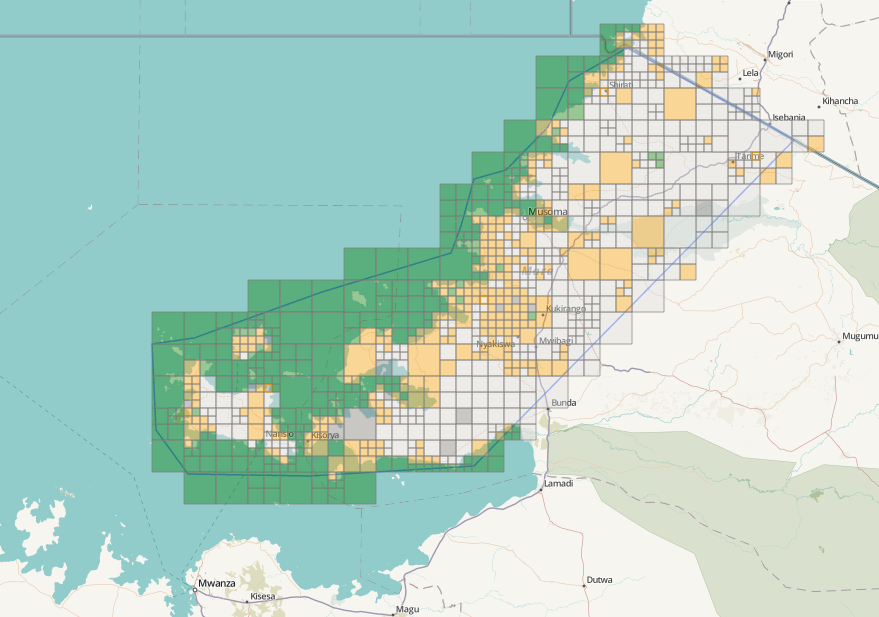
\includegraphics[scale=0.3]{figures/FixedByMe/taskingmanager.png}
    \caption{Project 2261- Tanzania Development, source: tasks.hotosm.org}
    \label{fig:project2261}
\end{figure} 

The OSM Tasking Manager has in the aftermath developed to other projects outside the HOT community. Especially import projects have had good leverage in this tool, more about this in chapter \ref{ch:importmethods}. Newer versions of this tool gave mappers the possibility to asynchronous communicate on tasks, making it easier to inform each other. Unfinished tasks often contain information from users who have been working on it with an explanation of what they mapped or what they didn't map. The Los Angeles building import, which started in 2015, developed the OSM Tasking Manager 2, adding new features to fit their needs. Adding possibilities for tasks being polygons and not grids. 

\begin{figure}[H]
    \centering
    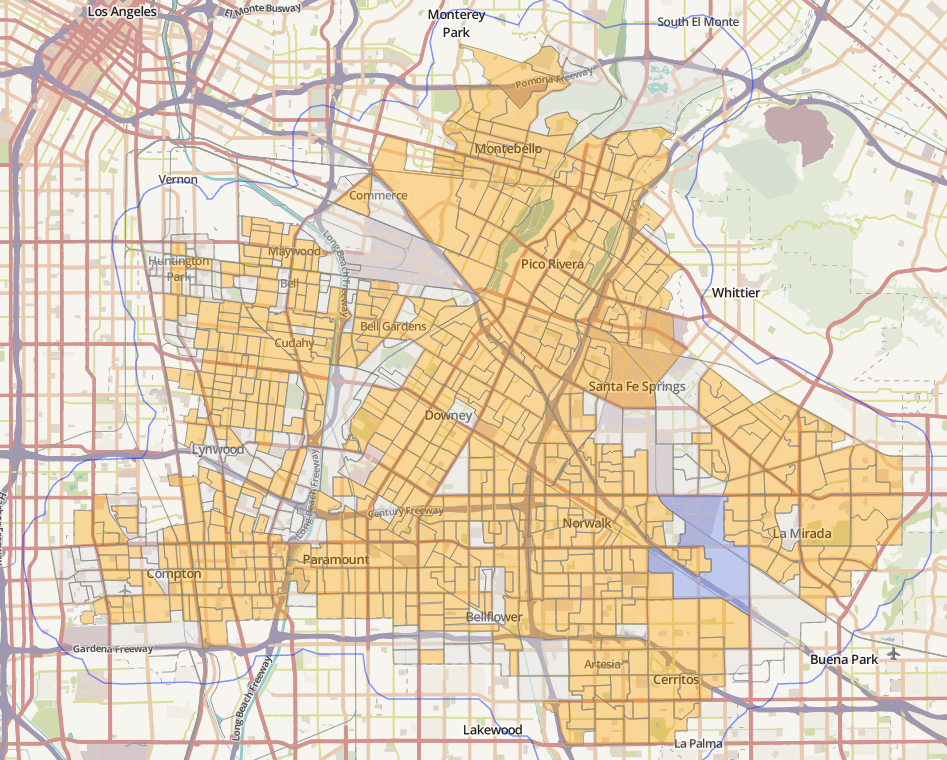
\includegraphics[scale=0.3]{figures/FixedByMe/taskingman2.png}
    \caption{Project 2 0- Southeast - LABuildings Import, source: labuildingsimport.com}
    \label{fig:project20}
\end{figure} 

An example of the OSM Tasking manager 2 used by the Los Angeles building import team is shown in figure \ref{fig:project20}. Notice that instead of grids they use polygons, dividing the tasks into a reasonable size using census block groups. More about this in subsection \ref{sec:importmicro}. 

\section{Other tools}
%To-fix, map-roulette 
There are other tools in OSM that use the micro-tasking method. They are designed for fixing bugs in the OSM database. Both Map-roulette and To-fix are examples of such tools and are listed as error detection tools on the OSM quality assurance wiki page. MapRoulette was created by Martijn van Exel and Serge Wroclawski and it's slogan is "\textit{Towards a better map, one bug at a time}". This tool has a gamified approach to fixing bugs, breaking common OSM data problems into micro-tasks. According it's founder Martijn it's become very popular mapping pastime for both amateur contributors and experienced mappers \cite{Exelvan2013}.  The tool break tasks that need fixing into challenges with a tutorial of how to best fix the issues in the challenge. It displays one issue at a time, once every issue in a task is fixed a new challenge is activated. Common issues are connectivity errors among ways, overlapping ways and equivalent ways \cite{OpenStreetMapk}. To-fix is a micro-tasking tool creates by MapBox and is very similar to MapRoulette. This tool breaks up big mapping jobs into smaller tasks that multiple people can work on asynchronously \cite{Lidman2014}. The tasks are queued up, then a group of mappers can do the tasks and track their progress. Tasks presented here are also commonly fixing overlapping and crossing highways. With To-fix issued can be fixed both through iD editor and JOSM editor. This tool do not give an introduction to the tasks like MapRoulette, making it more challenging knowing what. To-fix loads tasks much faster then MapRoulette who are quite slow. There are also bugs in MapRoulette for instance, half of the information text are not displayed because it's too long for the information box and the skip button do not work properly. Both solutions convey statistics presenting total fixed, skipped and marked as not error on each task. 

